\chapter{Metodología}

El objeto de estudio se encuentra localizado en la superficie rocosa de los centros arqueológicos y/o monumentos en el ciudad de Cusco, es así que para la detección y estimación del área que ocupa se tendrá en cuenta un enfoque pseudo-multiespectral dentro del espacio y rango visible [380nm - 760nm] para la obtención de imágenes RGB para su posterior procesamiento.

\section{Limitantes}
El enfoque propuesto restringe el espectro electromagnético al espectro visible para longitudes de onda entre correspondientes al rojo, verde y azul, dejando de lado así la radiación ultra violeta e infrarroja para el análisis de las muestras e imágenes capturadas, pudiendo aplicar de esta forma un método que no requiera de equipo de calidad y/o filtros de luz que incurren en un gasto considerable para su implementación.

Una vez establecidos los parámetros principales para el dispositivo receptor de luz y sus limitantes es necesario describir el espacio de estudio el cual se desarrollara en los centro arqueológico de Qenq'o y Sacsayhuaman pertenecientes a la ciudad del Cusco, siendo este lugar el preciso gracias al fácil acceso al patrimonio pétreo que lo conforman posibilitando la siguiente etapa que consiste en la recopilación de muestras (imágenes) de los muros afectados por el organismo simbionte (Liquen).

\section{Materiales y toma de muestras}
Para la toma de muestra y/o recolección de imágenes una vez en el sitio se harán uso de las cámaras de uso personal e integrados en los dispositivos móviles, la cual cuenta con las siguientes características:

\begin{itemize}
	\item 3 cámaras posteriores
	\item Resolución: 50MP f/1.8 + 5.0 MP f/2.2 + 2.0 MP f/2.4
	\item Espacio de luz detectable en el espectro RGB
\end{itemize} 

Y de la cual se puede destacar que el sensor de 50MP representa la cámara principal con una distancia focal de 1.8, mientras que la cámara de gran angular para un registro más amplio tiene una resolución de 5.0MP con una distancia focal de 2.2 y finalmente se tiene la cámara macro como 2.0MP con una distancia focal de 2.24 para la recepción de imágenes de alta resolución que se encuentran cerca al sensor y lente.

\begin{figure}[h]
	\centering
	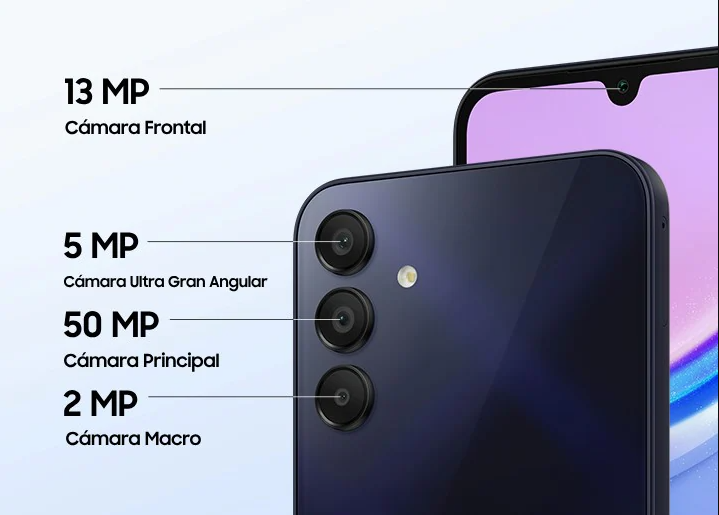
\includegraphics[width=0.5\linewidth]{media/especificaciones-camara}
	\caption{Especificación de las cámaras para la recepción de muestras}
	\label{fig:especificaciones-camara}
\end{figure}

En la imagen previa se puede apreciar la disposición de cada cámara y su resolución correspondiente para el dispositivo móvil a emplear.

Una vez definidos los materiales necesarios para la toma de muestras se realizará una visita in situ para realizar una recopilación de fotografías del material pétreo afectado, siendo así que para cada caso se tendrá en cuenta diferentes indicadores desde diferentes ángulos y para diferentes tipos de iluminación según lo requerido para una recolección satisfactoria.

\begin{figure}[h]
	\centering
	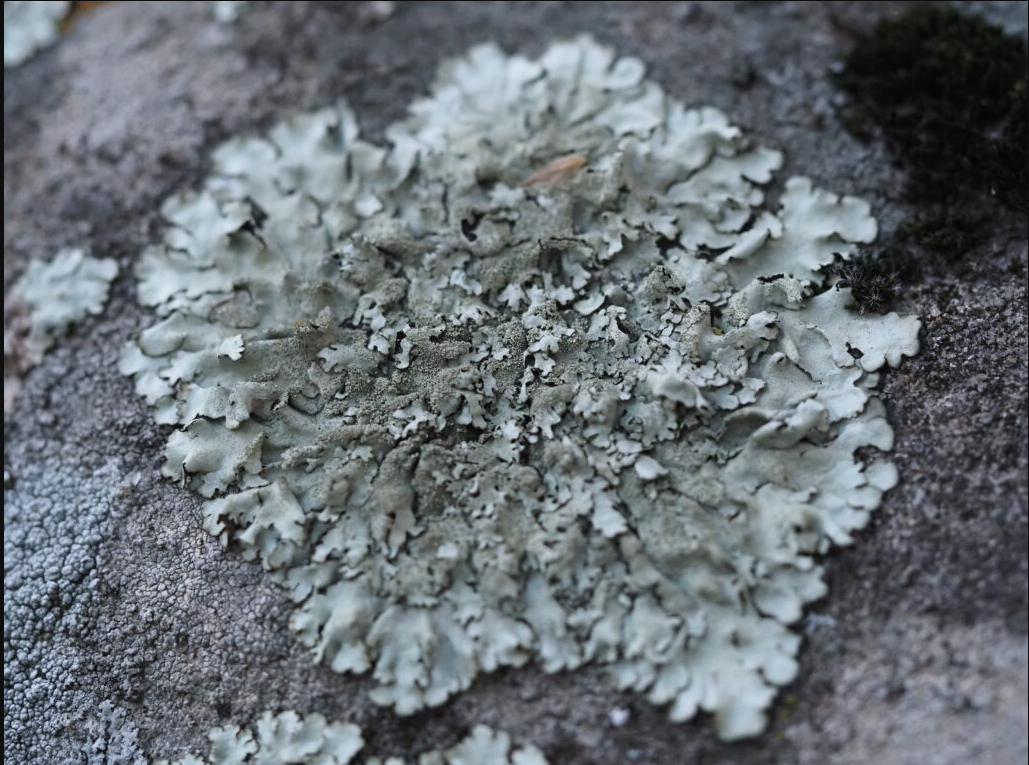
\includegraphics[width=0.5\linewidth]{./media/ejemplo-muestra-liquen}
	\caption{Muestrea pétrea afectada por un Liquen}
	\label{fig:ejemplo-muestra-liquen}
\end{figure}

En la imagen superior se tiene una muestra de ejemplo el cual consiste en una figura pétrea afectada para la cual se realizara el procesamiento  digital de la imagen para el análisis espectral utilizando para tal propósito la librería open-cv (Python) y relacionadas para un análisis en los diferentes modos de color que nos permitan segmentar las áreas de importancia afectadas por las especie orgánica.

\section{Procesamiento de muestras y segmentación mediante espectro}
Para el procesamiento de muestras se consideraran 2 puntos divididos en el preprocesamiento de la imagen y la detección del área afectada teniendo en cuenta para ello el enfoque teórico visto hasta el momento el actual procedimiento contemplará un esquema dinámico mediante el uso de diferentes modos de color entre los que destacaran

\begin{itemize}
	\item HSV (Hue,Saturation, Value)
	\item YUV (Luma, Croma (UV))
	\item YCbCr (Iluminación y cromado)
	\item LAB (Lightness, A, B)
\end{itemize}

u otros, considerando para caso la equalización entre otras transformaciones para la segmentación de la imagen según la reflectancia espectral de luz que los especímenes generan y que son captados por los sensores de las cámaras.

\section{Estimación del área afectada mediante segmentación}

Una vez procesadas las imágenes la siguiente etapa consta del reconocimiento del área afectada utilizando para ello un algoritmo de aprendizaje reforzado o Machine Learning mediante las tonalidades resultantes para cada pixel como resultado de la segmentación espectral aplicada mediante los modos de color y transformaciones ejecutadas, esto al no contemplar cierta uniformidad o linealidad para cada pixel, requiere de un modelo capaz de imitar el criterio humano agregando objetividad para aplicar cálculos precisos en función a la segmentación del espacio ocupado por el elemento orgánico híbrido.

\section{Calculo del área}

Para el calculo del área se pueden empe

\section{Métodos de Validación Propuestas}
Cuales serán las métricas utilizadas 